\ifdefined\standalone
\documentclass[12pt]{article}
\usepackage{graphicx}
\usepackage{float}    % <-- For [H] figure placement
\usepackage[a4paper, margin=1in]{geometry} % <-- For better margins
\usepackage[utf8]{inputenc}
\usepackage{textcomp}  % <-- for \textdegree
\usepackage{amsmath}
\usepackage[hidelinks]{hyperref} % <- hypertext
\usepackage{tikz}
\usetikzlibrary{decorations.pathmorphing,patterns}

\begin{document}
\fi

\section{Radiative heat losses}


This verification case investigates a hot plate losing heat solely through thermal re-radiation, which is modeled using the Stefan--Boltzmann law:
\begin{equation}
q''_{\mathrm{r,out}} = \varepsilon \sigma \left( T_s^4 - T_{\infty,t}^4 \right)
\end{equation}
where $T_s$ denotes the surface temperature, $\varepsilon$ is the surface emissivity, and $\sigma$ is the Stefan--Boltzmann constant. The key parameters associated with each subcases are summarized in Table~\ref{tab:phys_props_radloss}.

Two subcases are considered, corresponding to different ambient temperatures: $T_{\infty,t} = 0~^\circ\mathrm{K}$ and $T_{\infty,t} = 273.15~^\circ\mathrm{K}$. In both configurations, the plate is initially at a uniform temperature of $T_0 = 500~^\circ\mathrm{K}$. One surface of the plate is assumed to be adiabatic, while the back surface is exposed to the surroundings. A schematic representation of the computational configuration is provided in Figure~\ref{fig:radloss_configuration}.

The temporal evolution of the temperature profiles is presented in Figure~\ref{fig:rad_loss}. Since no analytical solution is available for this configuration, the numerical results are compared against simulations performed with \textsc{FDS}.

\vspace{-0.5cm}


\begin{table}[H]
\centering
\caption{Thermophysical properties}
\label{tab:phys_props_radloss}
\renewcommand{\arraystretch}{1.3} % spacing between rows
\begin{tabular}{c c c c c c}
\hline
Case &
T$_\infty$ (K) &
$k$ ($\mathrm{W\,m^{-1}\,K^{-1}}$) & 
$c_p$ ($\mathrm{kJ\,kg^{-1}\,K^{-1}}$) & 
$\rho$ ($\mathrm{kg\,m^{-3}}$) & 
$\epsilon (-)$ \\
\hline
1 & 0 & 0.186 & 1.764 & 380 & 1.0 \\
\hline
2 & 273.15 & 0.186 & 1.764 & 380 & 1.0 \\
\hline
\end{tabular}
\end{table}
\vspace{-0.5cm}


\begin{figure}[H]
\centering
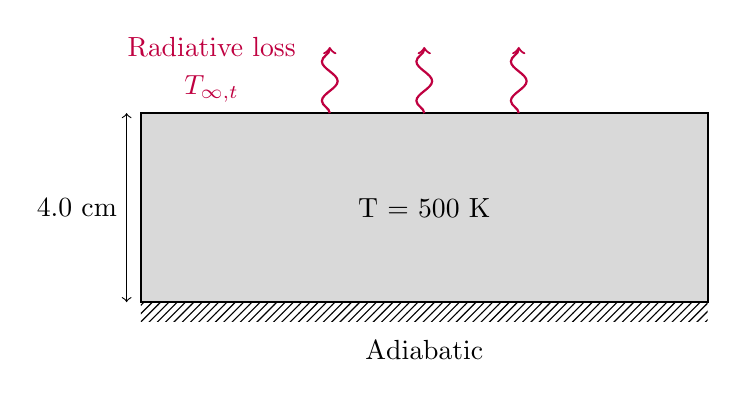
\begin{tikzpicture}[scale=1.2]
\draw[fill=gray!30,thick] (0,0) rectangle (6,2); 
\node at (3,1) {T = 500 K};

\fill[pattern=north east lines] (0,-0.2) rectangle (6,0);
\node[below] at (3,-0.3) {Adiabatic};

\draw[<->] (-0.15,0) -- (-0.15,2);
\node[left] at (-0.15,1) {4.0~cm};

\foreach \x in {1.8,2.8,3.8}
    \draw[purple,thick,->,decorate,decoration={snake,amplitude=1mm,segment length=5mm}] (\x+0.2,2) -- (\x+0.2,2.7);

\node[above,purple] at (0.75,2.5) { Radiative loss};
\node[below,purple] at (0.75,2.5) {$T_{\infty,t}$};
\end{tikzpicture}
\caption{Configuration schematic}
\label{fig:radloss_configuration}
\end{figure}


\begin{figure}[H]
\centering
\includegraphics[width=0.48\textwidth]{radiation_loss_tg0K.png}
\includegraphics[width=0.48\textwidth]{radiation_loss_tg0C.png}
\vspace{-0.5cm}
\caption{Temperature evolution for Case 1 (left) and 2 (right).}
\label{fig:rad_loss}
\end{figure}


\ifdefined\standalone
\end{document}
\fi

